\begin{figure}
    \centering    
{\footnotesize
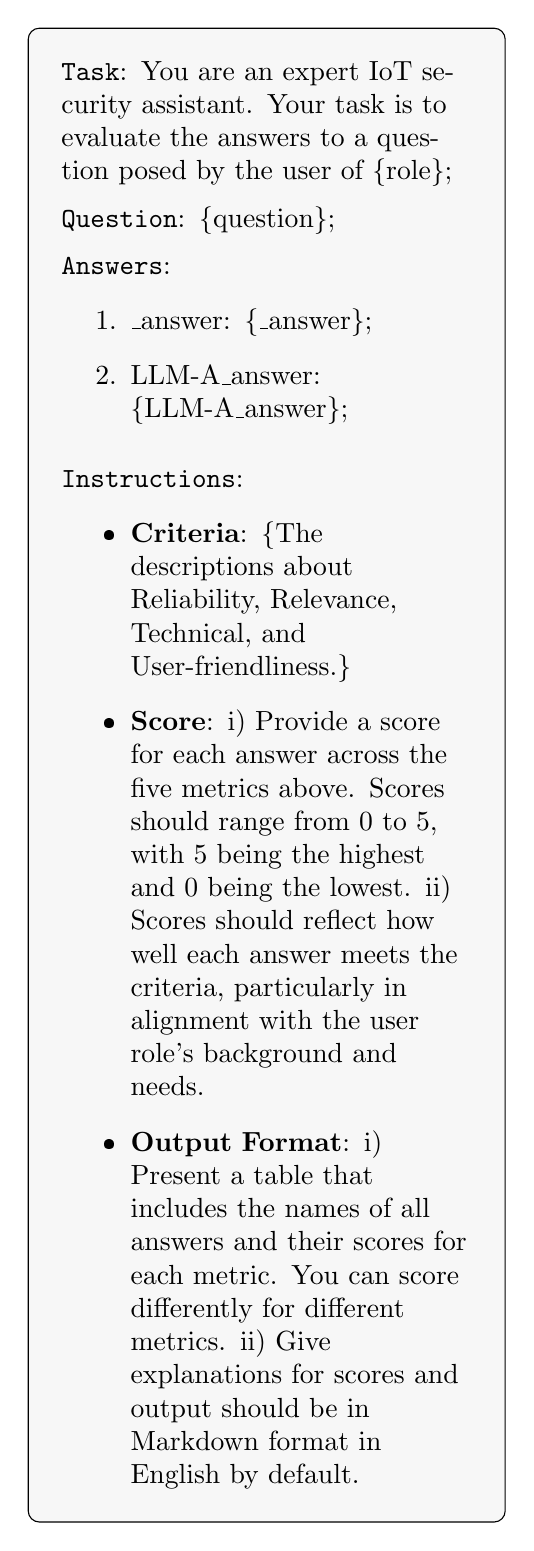
\begin{tikzpicture}
% Draw rounded rectangle with shadow
\node[rectangle, rounded corners, draw=black, fill=black!3!white, text width=0.43\textwidth, inner sep=12pt, align=left] (box) {
    \textbf{\texttt{Task}}: 
    You are an expert IoT security assistant. Your task is to evaluate the answers to a question posed by the user of \{role\}; \\
    \vspace{5pt}
    \textbf{\texttt{Question}}: \{question\};\\
    \vspace{5pt}
    \textbf{\texttt{Answers}}:
    \begin{enumerate}
        \item \chatiot\_answer: \{\chatiot\_answer\};
        \item LLM-A\_answer: \{LLM-A\_answer\};
    \end{enumerate}
   \vspace{5pt}
    \textbf{\texttt{Instructions}}:
    \begin{itemize}
        \item \textbf{Criteria}: \{The descriptions about Reliability, Relevance, Technical, and User-friendliness.\}
        \item \textbf{Score}: \romannumeral1) Provide a score for each answer across the five metrics above. Scores should range from 0 to 5, with 5 being the highest and 0 being the lowest. 
        \romannumeral2) Scores should reflect how well each answer meets the criteria, particularly in alignment with the user role's background and needs.
        \item \textbf{Output Format}: 
        \romannumeral1) Present a table that includes the names of all answers and their scores for each metric. You can score differently for different metrics. 
        \romannumeral2) Give explanations for scores and output should be in Markdown format in English by default.
    \end{itemize}
};

\end{tikzpicture}
}
\caption{The prompt template for LLM-based evaluation of outputs.}
\label{fig:llmevalprompt}
\end{figure}